% !TeX program = lualatex
% =============================================================================
%  AB Power Meter Monitor - Release 1.6.2 Technical Manual
%  File     : docs/AB_Power_Meter_Manual.tex
%  Version  : 1.6.2 (matches ab_power_meter_monitor.py 1.6.2)
%  Author   : William W. Wallace, NRAO/GBO
%  Created  : 2026-10-26     Modified: 2026-10-26
%  Build    : latexmk -lualatex AB_Power_Meter_Manual.tex   (or: lualatex x2)
%  Licence  : GPL-3.0-or-later (same as the software it documents)
%  Revision history
%    1.6.2  2026-10-26  Windows operation (files open in Excel, Ctrl+Break) and the
%                       Windows test kit; verification updated.
%    1.6.1  2026-10-26  Windows memory release (Sec. osrelease), busy-writer
%                       duplicate-row race, Windows (Wine) verification.
%    1.6.0  2026-10-26  First LuaLaTeX manual (release 1.6.0 findings, design,
%                       configuration, verification, module review).
% =============================================================================
\documentclass[11pt,a4paper]{article}

% --- Engine-native fonts and maths (LuaLaTeX) --------------------------------
\usepackage{fontspec}
\usepackage{unicode-math}
\setmainfont{Latin Modern Roman}
\setsansfont{Latin Modern Sans}
\setmonofont{DejaVu Sans Mono}[Scale=0.84]
\setmathfont{Latin Modern Math}

% --- Layout and typography ------------------------------------------------------
\usepackage[margin=2.2cm,headheight=14pt]{geometry}
\usepackage{microtype}
\usepackage{xcolor}
\usepackage{graphicx}
\usepackage{booktabs,longtable,tabularx,array}
\usepackage{enumitem}
\usepackage{caption}
\usepackage{fancyhdr}
\usepackage{listings}
\usepackage{tikz}
\usetikzlibrary{arrows.meta,positioning,fit,backgrounds}
\usepackage{pgfplots}
\pgfplotsset{compat=1.18}
\usepackage{siunitx}

% --- PDF bookmarks (outline pane opens on load) and links ------------------------
\usepackage[bookmarks=true,bookmarksopen=true,bookmarksopenlevel=2,
            bookmarksnumbered=true,colorlinks=true,linkcolor=blue!50!black,
            urlcolor=blue!50!black,citecolor=blue!50!black,
            pdfpagemode=UseOutlines]{hyperref}
\usepackage{bookmark}
\hypersetup{pdftitle={AB Power Meter Monitor 1.6.2 - Technical Manual},
            pdfauthor={William W. Wallace, NRAO/GBO},
            pdfsubject={Release 1.6.2: RAM flush (Linux and Windows), Windows operation, native .vszh5 appending, Python 3.12},
            pdfkeywords={Allen-Bradley, power meter, Veusz, vszh5, HDF5, Prometheus, PySide6}}

% --- Helpers -------------------------------------------------------------------------
\newcommand{\code}[1]{\texttt{\detokenize{#1}}}
\definecolor{codebg}{RGB}{246,246,246}
\lstset{basicstyle=\ttfamily\small,backgroundcolor=\color{codebg},frame=single,
        rulecolor=\color{black!25},columns=fullflexible,keepspaces=true,
        breaklines=true,showstringspaces=false,xleftmargin=4pt,xrightmargin=4pt}
\setlist{itemsep=2pt,topsep=4pt}
\pagestyle{fancy}
\fancyhf{}
\fancyhead[L]{\small AB Power Meter Monitor 1.6.2}
\fancyhead[R]{\small Technical Manual}
\fancyfoot[C]{\small\thepage}
\renewcommand{\arraystretch}{1.15}

\begin{document}

% =============================================================================
\begin{titlepage}
  \centering
  \vspace*{2.5cm}
  {\Huge\bfseries AB Power Meter Monitor\par}
  \vspace{0.4cm}
  {\LARGE Release 1.6.2 --- Technical Manual\par}
  \vspace{0.8cm}
  {\large Allen-Bradley 1403 site power-meter poller, data logger, GUI\\
  and Prometheus exporter for NRAO / Green Bank Observatory\par}
  \vspace{1.5cm}
  \begin{tabular}{ll}
    \toprule
    Component & Version \\
    \midrule
    \code{ab_power_meter_monitor.py} & 1.6.2 \\
    \code{vszh5_writer.py} & 0.0.18 \\
    \code{ab_prometheus_exporter.py} & 0.1.1 \\
    \code{ab_meter_caller.py} & 1.3.0 \\
    Python (primary, tested) & 3.12.3 \\
    Windows Python (tested under Wine 9.0) & 3.12.15 \\
    Veusz (viewer, verified) & 4.2.1 \\
    \bottomrule
  \end{tabular}
  \vfill
  {\large William W. Wallace\\NRAO / Green Bank Observatory\\
   \href{mailto:wwallace@nrao.edu}{wwallace@nrao.edu}\par}
  \vspace{0.6cm}
  {\large 26 October 2026\par}
\end{titlepage}

\tableofcontents
\clearpage

% =============================================================================
\section{Summary}
Release 1.6.0 makes the memory protection of the monitor work in the GUI and
in headless operation, replaces the Veusz output with native \code{.vszh5}
documents that are appended in place on every poll, fixes a FITS defect that
multiplied rows on every rewrite, and corrects the Prometheus exporter so it
never re-exports stale readings. Python~3.12 is the primary, tested target;
the source remains at the Python~3.7 language level. Every defect below was
first reproduced against an offline emulator of the meter web pages and then
verified fixed (Section~\ref{sec:verification}).

Release 1.6.1 makes the flush hand the freed memory back to \emph{Windows}
as well (1.6.0 did so only on Linux), Section~\ref{sec:osrelease}, and fixes a
race in which a forced write (flush, Save~Now, stop) waiting for a busy writer
could send the same rows twice (Section~\ref{sec:fits}). The race was found by
running the test-suite on a Windows build of Python~3.12.

Release 1.6.2 makes Windows operation robust: an output file held open by
another program (Excel) no longer produces an error per table per poll, and
its rows are kept or written to rescue files that are merged back; Ctrl+Break
now stops the headless monitor and the exporter gracefully. A Windows test
kit (Section~\ref{sec:windows}) runs every check on a Windows PC.

% =============================================================================
\section{Findings: RAM flush}\label{sec:ramflush}
\subsection{Why the flush did not protect the GUI}
The 1.5.5 flush logic only manages \code{TIME_SERIES_STORE}. In the GUI the
dominant memory growth was elsewhere, so clearing the store could not help:

\begin{enumerate}
  \item \textbf{Preview tabs leaked every poll.} \code{_populate_plot_tabs()}
        called \code{QTabWidget.clear()} and rebuilt every tab. Qt documents
        that \code{clear()} and \code{removeTab()} do \emph{not} delete the page
        widgets~\cite{qt_qtabwidget}; each poll therefore left about 70 widgets
        plus their full-size pixmaps alive. Measured on the original code at a
        2\,s period: \num{1507} $\rightarrow$ \num{2947} $\rightarrow$ \num{4387}
        live widgets and \SI{436}{\mebi\byte} $\rightarrow$ \SI{691}{\mebi\byte}
        $\rightarrow$ \SI{946}{\mebi\byte} RSS at \SIlist{0;45.8;91.2}{\second}
        (Fig.~\ref{fig:gui-leak}).
  \item \textbf{The log console grew without bound} (\code{QTextEdit},
        DEBUG level, one line per page fetch).
  \item \textbf{The store-size trigger never cleared anything.} In headless mode
        \code{should_flush()} rewrote the files but left the store intact; the
        GUI never evaluated it at all. Only the system-RAM-\% trigger cleared.
  \item \textbf{The system-RAM-\% trigger mis-fired.} It is system-wide: when
        other processes held the RAM, the monitor flushed and cleared its store
        on \emph{every} poll without freeing anything significant.
  \item \textbf{Freed memory was not returned to the operating system.}
        \code{gc.collect()} frees objects, but the allocator keeps the pages,
        so RSS (and the RAM \%) stayed high after a flush.
  \item \textbf{FITS rewrites multiplied rows} (Section~\ref{sec:fits}); with
        FITS enabled the GUI exhausted memory in minutes regardless of any flush.
  \item \textbf{GUI-thread saturation.} About 40 preview PNGs were rendered
        on the GUI thread every poll and Poll~Now ran the whole poll on it.
\end{enumerate}

\subsection{What 1.6.0 does}
\begin{itemize}
  \item Preview tabs are created once per plot and updated in place; tabs that
        disappear are \code{deleteLater()}'d. Only the visible tab is rendered,
        min/max decimated to \code{PREVIEW_MAX_POINTS} per series, and the
        pixmap of a tab is released when the user leaves it.
  \item The console is a \code{QPlainTextEdit} with \code{maximumBlockCount}
        \cite{qt_qplaintextedit}, fed from any thread through a queued signal.
  \item Polling, persistence and flushing run in an acquisition worker thread
        (\code{QThread}); Save~Now, Flush~RAM~Now and Open~in~Veusz are
        executed by that worker between polls, so they never race it.
  \item One flush function, \code{perform_ram_flush()}, serves the GUI, the
        headless loop and the caller. It persists every enabled output, waits
        for the writes, drops only rows that \emph{every} output confirmed, and
        then returns the freed memory to the operating system: \code{malloc_trim(0)}
        on Linux~\cite{malloc_trim}, heap decommit and working-set trim on
        Windows since 1.6.1 (Section~\ref{sec:osrelease}).
  \item Triggers are store estimate, process RSS, system RAM \% and free RAM,
        with a minimum interval and a minimum store size for the system-wide
        triggers (Eq.~\ref{eq:trigger}).
\end{itemize}

\subsection{Store estimate and trigger}
For table $i$ with $n_i$ rows and $k_i$ parameters, the store estimate in bytes
is evaluated in $O(\text{tables})$ every poll:
\begin{equation}
  B = \sum_i n_i\,\bigl(32\,k_i + 144\bigr),\label{eq:store}
\end{equation}
32\,B being one float object (24\,B) plus its list slot (8\,B) and 144\,B per
row the timestamp string, sequence number and Unix time. Against an exact object
walk the estimate was within 1\,\% (\SI{5.54}{\mebi\byte} vs.
\SI{5.57}{\mebi\byte}; \SI{22.16}{\mebi\byte} vs. \SI{21.92}{\mebi\byte}).
With $\Delta t$ the time since the last flush, an automatic flush happens when
\begin{equation}
  F = E \wedge \bigl(\Delta t \ge T_{\min}\bigr) \wedge
      \Bigl[\,(B > B_{\max}) \;\vee\; \bigl(B \ge B_{\min} \wedge
      (R > R_{\max} \;\vee\; P \ge P_{\max} \;\vee\; M_{\text{free}} < M_{\min})\bigr)\Bigr],
  \label{eq:trigger}
\end{equation}
where $E$ is \code{ENABLE_RAM_FLUSH}, $T_{\min}$
\code{MEM_FLUSH_MIN_INTERVAL_SEC}, $B_{\max}$ \code{MEM_FLUSH_THRESHOLD_MB},
$B_{\min}$ \code{MEM_MIN_STORE_MB_FOR_CLEAR}, $R$ the process RSS, $P$ the
system RAM use and $M_{\text{free}}$ the free RAM.

\subsection{Returning memory to the operating system (1.6.1)}\label{sec:osrelease}
Dropping rows frees Python objects, but three layers below keep memory:
CPython's \code{pymalloc} returns a 1\,MiB arena (with \code{VirtualFree} or
\code{munmap}) only when every object in it is free~\cite{cpython_obmalloc};
the C heap keeps freed blocks committed; and on Windows even released pages
stay in the process's \emph{working set} --- Task Manager's ``Memory''
column --- until the memory manager trims it. 1.6.0 handled only Linux, so on
Windows a flush emptied the store but Task Manager showed no drop.
With \code{MEM_RETURN_TO_OS = 1}, \code{return_memory_to_os()} now runs after
every flush:

\begin{center}
\begin{tabularx}{\linewidth}{@{}p{0.17\linewidth}p{0.36\linewidth}>{\raggedright\arraybackslash}X@{}}
\toprule
OS & Call & Effect \\
\midrule
Linux (glibc) & \code{malloc_trim(0)} & free heap pages returned to the kernel~\cite{malloc_trim} \\
Windows 8.1+ & \code{HeapSetInformation(NULL,}\newline\hspace*{1em}\code{HeapOptimizeResources,}\newline\hspace*{1em}\code{{Version=1, Flags=0})} & every heap with a low-fragmentation heap: caches optimised, memory decommitted if possible~\cite{ms_heapsetinfo}; the call Firefox makes under memory pressure~\cite{moz_1553296} \\
Windows & \code{EmptyWorkingSet(}\newline\hspace*{1em}\code{GetCurrentProcess())}\newline(\code{MEM_TRIM_WORKING_SET}) & removes as many pages as possible from the working set~\cite{ms_emptyws}; pages still in use fault back in on their next access \\
not used & \code{_heapmin()} & in the Universal CRT this is only \code{HeapCompact(__acrt_heap, 0)}~\cite{reactos_heapmin}, which ``does not compact the heap any further'' on a normal system~\cite{ms_heapcompact} \\
\bottomrule
\end{tabularx}
\end{center}

The Windows functions are bound once through private \code{ctypes.WinDLL}
instances with explicit \code{HANDLE} and \code{SIZE_T} argument types (the
\code{ctypes} default C \code{int} would truncate 64-bit handles), the release
is serialised by a non-blocking lock, runs outside the persistence lock and
never raises into the poll loop. On Windows two numbers matter: the working
set $W$ (\code{psutil} \code{rss}, Task Manager ``Memory'') and the commit
charge $C$ (private bytes, \code{psutil} \code{vms}, Task Manager ``Commit
size''). With $D$ the memory the heaps could decommit,
\begin{equation}
  C_{\text{after}} = C_{\text{before}} - D, \qquad
  W_{\text{after}} \approx W_{\text{touched}} \le C_{\text{after}},
  \label{eq:winrelease}
\end{equation}
where $W_{\text{touched}}$ is the memory the process uses again before the
next measurement. Both values are printed in the flush log and the GUI.

\medskip\noindent Measured with \code{tests/test_memory_release.py}: a store of
\num{3000000} values (estimate \SI{98.4}{\mebi\byte}) is filled and flushed.
\begin{center}
\begin{tabular}{@{}lrrrl@{}}
\toprule
 & \multicolumn{3}{c}{RSS (MiB)} & \\
\cmidrule(lr){2-4}
Run & idle & filled & flushed & OS step \\
\midrule
Linux, Python 3.12.3 & 64 & 180 & 70 & \code{malloc_trim}: 96 $\rightarrow$ 70 \\
Linux, Python 3.8.20 & 51 & 169 & 54 & \code{malloc_trim}: 80 $\rightarrow$ 54 \\
Windows Python 3.12.15 (Wine) & 350 & 466 & 364 & both calls succeed$^{\ast}$ \\
GUI soak, Flush RAM Now (Linux) & \multicolumn{3}{c}{239 $\rightarrow$ 220} & \code{malloc_trim} \\
\bottomrule
\end{tabular}

\smallskip
{\footnotesize $^{\ast}$Wine runs the Windows code paths but not the Windows
memory manager; the Windows drop measured there comes from \code{pymalloc}
freeing whole arenas.}
\end{center}

% =============================================================================
\section{Findings: iterative .vszh5 writing}\label{sec:vszh5}
\subsection{How 1.5.5 wrote Veusz files}
\begin{itemize}
  \item It required the \code{veusz} Python package and drove
        \code{veusz.embed.Embedded}, which starts a Veusz process and rebuilds
        the \emph{whole} document from the in-memory store on every save.
        Nothing was appended: the document could only reflect what was still in
        RAM.
  \item Consequently, every RAM flush had to produce a separate timestamped
        snapshot file, and the final file after a flushed run held only the last
        window. A long run became a scattered set of partial documents.
  \item Headless runs wrote Veusz only at the end of the run (and optionally at a
        flush); a crash lost the whole document. Caller mode rebuilt the full
        document, through a new Veusz process, on every poll.
  \item Dataset names were cut to 64 characters, so long parameter names could
        collide and silently overwrite each other.
\end{itemize}

\subsection{How 1.6.0 writes them}
\code{vszh5_writer.py} 0.0.18 adds \code{VeuszAppender}, which opens an
existing document \code{'r+'} and grows it; the monitor uses it for one
document per meter, \code{ABMeter_<ip>.vszh5}, appended on every poll:
\begin{itemize}
  \item per table a date dataset \code{<octet>_dt_<table>} and one numeric
        dataset per parameter, collision-free and never truncated;
  \item datasets are chunked (1024 rows), resizable and \emph{uncompressed}:
        a partly filled compressed chunk that grows is moved, leaving dead space,
        so compression would bloat a file appended every 30\,s~\cite{h5py_datasets};
  \item the fill value is NaN, so rows reserved by a resize but never written
        (power loss mid-append) read back as gaps, not zeros; on the next append
        columns are padded or truncated back to the length of the time axis;
  \item a parameter that appears later is back-filled with NaN; the Veusz page
        script (per-table grid pages, per-unit overlay pages) is rewritten only
        when datasets are added;
  \item the table$\to$dataset index lives in \code{/VszAppend}; Veusz~4.2.1
        reads only \code{/Veusz} (confirmed in its \code{loadHDF5Doc}
        \cite{veusz_src}), so appending resumes after a restart;
  \item when a reader holds the HDF5 file lock (Veusz while loading) the rows
        stay in memory for the next poll; if they must land now (flush, stop) a
        standalone rescue document is written; an unreadable file is moved aside
        and a new one started; rollover at \code{VSZH5_MAX_FILE_MB}.
\end{itemize}
Each append writes only the new rows: the cost per poll is
$O(\text{new rows})$, independent of the document size. The appended documents
load and render in real Veusz~4.2.1 (all 23 pages plus the PDF,
Fig.~\ref{fig:veusz}).

\begin{figure}[ht]
  \centering
  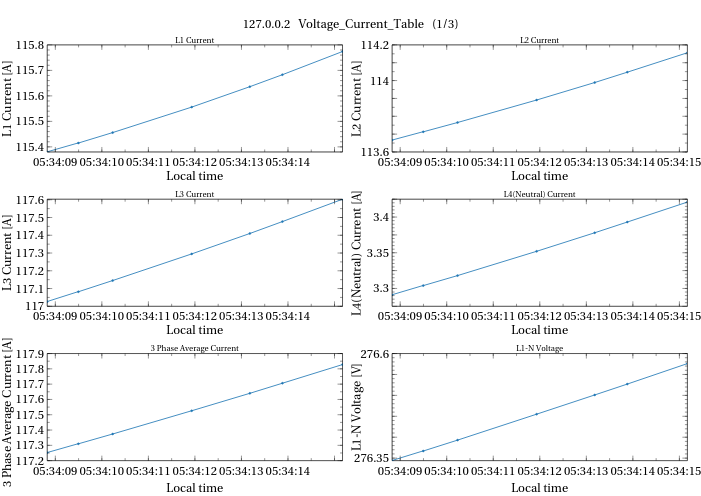
\includegraphics[width=0.49\linewidth]{figures/veusz_grid_page.png}\hfill
  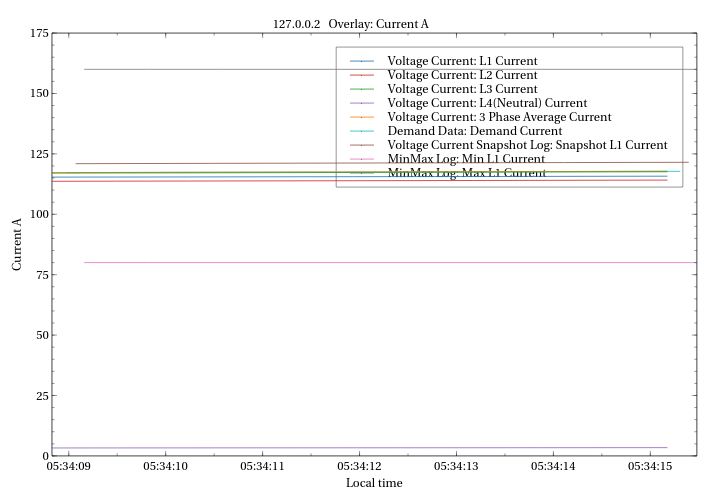
\includegraphics[width=0.49\linewidth]{figures/veusz_overlay_page.png}
  \caption{Pages of an appended \code{.vszh5} rendered by real Veusz 4.2.1:
  per-table grid page (left) and overlay page (right), emulator data.}
  \label{fig:veusz}
\end{figure}

% =============================================================================
\section{Other defects fixed}\label{sec:fits}
\begin{description}[style=nextline]
  \item[FITS row multiplication] \code{EXTNAME = tname[:8]} made
        \code{Voltage_Current_Table}/\code{Voltage_Current_Snapshot_Log_Table}
        and \code{Diagnostic_Table}/\code{Diagnostic_Table_Extended} collide;
        the reader merged the two HDUs and each rewrite copied both tables' rows
        into both HDUs (Fig.~\ref{fig:fits}). Same-second timestamp
        de-duplication also dropped genuine rows. 1.6.0 uses the full table
        name, separates old files by \code{TBLNAME}, adds \code{EPOCH_UTC},
        and writes atomically (temporary file, then \code{os.replace}).
  \item[CSV / Markdown append] In append mode across runs, row counting mixed old
        and current rows and writing stopped after the first poll. Writers now
        keep per-row sequence cursors.
  \item[Exporter] Re-exported a dead meter's last values; \code{samples_total}
        plateaued (not a valid counter~\cite{prom_exporters}). See
        Section~\ref{sec:exporter}.
  \item[Concurrency] \code{ALL_DEVICE_DATA} was rebuilt while the GUI iterated
        it; now swapped under a lock.
  \item[Duplicates] Duplicate IPs polled one meter from two threads; duplicate
        parameter names overwrote each other (now \texttt{Name [\#N]}).
  \item[Python 3.12] \code{datetime.utcnow()} is deprecated~\cite{py_datetime,py312};
        replaced by timezone-aware UTC.
  \item[Service wrapper] \code{POLL_INTERVAL} was read but never passed on.
  \item[Requirements] \code{qtpy} (imported by the GUI) was missing.
  \item[Duplicate rows after a busy writer (1.6.1)] 1.6.0 advanced a writer's
        cursors in a future done-callback. \code{concurrent.futures} wakes the
        threads blocked in \code{result()} \emph{before} it runs the
        done-callbacks~\cite{cpython_futures}, so a forced persist that waited
        for a busy writer could read the old cursor and send rows a second
        time; every writer appends or merges without de-duplication. Found as
        extra XLSX rows when the suite ran on Windows Python (slower writes);
        possible on any OS. Fixed in Section~\ref{sec:cursors}.
\end{description}

\begin{figure}[ht]
  \centering
  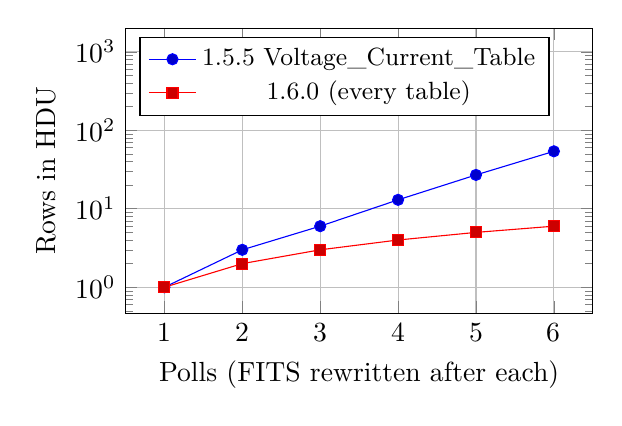
\begin{tikzpicture}
    \begin{axis}[width=0.62\linewidth,height=5.2cm,xlabel={Polls (FITS rewritten after each)},
                 ylabel={Rows in HDU},ymode=log,log basis y=10,ymax=2000,
                 legend style={at={(0.03,0.97)},anchor=north west,font=\small},
                 grid=major,xtick={1,...,6}]
      \addplot+[mark=*] coordinates {(1,1)(2,3)(3,6)(4,13)(5,27)(6,54)};
      \addlegendentry{1.5.5 Voltage\_Current\_Table}
      \addplot+[mark=square*] coordinates {(1,1)(2,2)(3,3)(4,4)(5,5)(6,6)};
      \addlegendentry{1.6.0 (every table)}
    \end{axis}
  \end{tikzpicture}
  \caption{FITS rows per HDU after successive rewrites (emulator, measured).}
  \label{fig:fits}
\end{figure}

% =============================================================================
\section{Architecture}
\subsection{Threads}
\begin{figure}[ht]
\centering
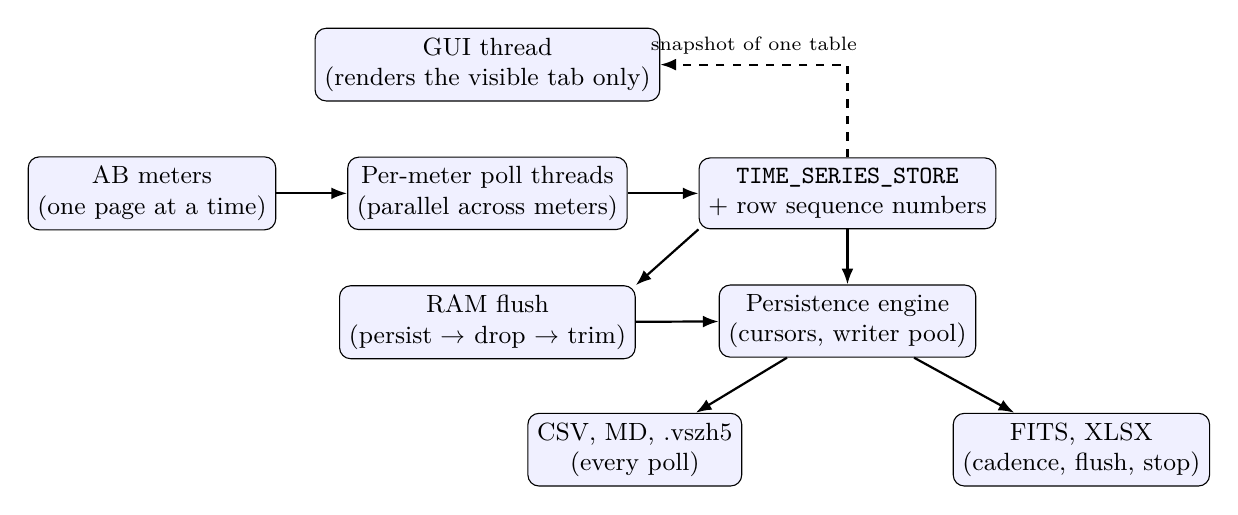
\begin{tikzpicture}[node distance=7mm and 9mm,
  box/.style={draw,rounded corners,fill=blue!6,align=center,minimum height=9mm,font=\small},
  arr/.style={-{Latex[length=2mm]},thick}]
  \node[box] (meters) {AB meters\\ \small(one page at a time)};
  \node[box,right=of meters] (poll) {Per-meter poll threads\\(parallel across meters)};
  \node[box,right=of poll] (store) {\code{TIME_SERIES_STORE}\\+ row sequence numbers};
  \node[box,above=of poll] (gui) {GUI thread\\(renders the visible tab only)};
  \node[box,below=of store] (persist) {Persistence engine\\(cursors, writer pool)};
  \node[box,below=of poll] (flush) {RAM flush\\(persist $\rightarrow$ drop $\rightarrow$ trim)};
  \node[box,below left=of persist,xshift=12mm] (files) {CSV, MD, .vszh5\\(every poll)};
  \node[box,below right=of persist,xshift=-12mm] (full) {FITS, XLSX\\(cadence, flush, stop)};
  \draw[arr] (meters) -- (poll);
  \draw[arr] (poll) -- (store);
  \draw[arr] (store) -- (persist);
  \draw[arr] (persist) -- (files);
  \draw[arr] (persist) -- (full);
  \draw[arr] (store.south west) -- (flush.north east);
  \draw[arr] (flush) -- (persist);
  \draw[arr,dashed] (store.north) |- node[pos=0.75,above,font=\scriptsize]{snapshot of one table} (gui.east);
\end{tikzpicture}
\caption{Data flow. The acquisition worker (GUI) or the headless loop runs the
poll, the persistence and the flush in one thread; the GUI thread only reads
snapshots of the table it displays.}
\end{figure}

\subsection{Persistence by sequence cursors}\label{sec:cursors}
Each stored row $r$ receives a process-wide increasing sequence number $s_r$.
Every writer $w$ keeps, per output folder and per (meter, table), the highest
sequence number it persisted, $c_w$. A persist call copies once, under the
store lock, the rows with $s_r > \min_w c_w$, and hands each writer the rows
with $s_r > c_w$. A writer's cursor moves only after its write succeeded, and a
writer whose previous write is still running is skipped (never two writes to
one file). Since 1.6.1 the cursor is advanced inside the writer task, before
its future completes, and each writer's cursor is read only after its previous
write is confirmed done at time $t_{\text{done}}$, so the rows handed to $w$ are
\begin{equation}
  R_w = \{\, r : s_r > c_w(t_{\text{done}}) \,\},
\end{equation}
which cannot contain a row already written (1.6.0 could read $c_w$ before the
callback that advanced it had run). A flush may drop row $r$ only if
\begin{equation}
  s_r \le \min_{w \in W} c_w ,
\end{equation}
with $W$ the enabled outputs, which is the formal statement of
``no row is dropped before every output has written it''.

% =============================================================================
\section{Windows operation (1.6.2)}\label{sec:windows}
\subsection{Output files held open by another program}
Excel keeps an open CSV or workbook locked against writes by other programs.
In Windows terms the file was opened with a share mode that lets others read
but not write; a later open for writing fails with a sharing
violation~\cite{ms_createfile}, which Python raises as
\code{PermissionError} (Win32 errors 5, 32 or 33). 1.6.1 logged an ERROR for
every table on every poll in that state, and a RAM flush could not drop the
rows. 1.6.2 treats the file as \emph{in use}:
\begin{itemize}
  \item one WARNING per file per 10 minutes; the writer's cursor does not
        move, so the rows stay in memory and are written once the file is
        closed;
  \item a forced persist (flush, Save~Now, stop) writes them to
        \code{<file>_<YYYYmmdd_HHMMSS>[_N]_rescue.csv} (or \code{.md}), so the
        flush can still free the memory;
  \item the next successful write first merges the rescue files, ordered by
        (time stamp, counter): each is renamed to \code{.merging} before its
        rows are copied, so a merge is never repeated even if deleting the
        file afterwards fails;
  \item new Markdown rows after a merged rescue section start a
        ``(continued)'' section.
\end{itemize}
FITS, XLSX and \code{.vszh5} already kept their rows or wrote rescue files.

\subsection{Stopping with Ctrl+Break}
On Windows \code{SIGTERM} sent by another process is \code{TerminateProcess}
and cannot be handled~\cite{py_subprocess}; supervisors send
\code{CTRL_BREAK_EVENT} to the process group instead, which reaches only
processes sharing the sender's console~\cite{ms_ctrlevent}. The monitor
(1.6.2) and the exporter (0.1.1) now handle \code{SIGBREAK} like
\code{SIGINT}/\code{SIGTERM}: stop after the current page, then the final
writes. Before, Ctrl+Break killed them without the final FITS/XLSX writes.

\subsection{Windows test kit}
\code{windows/} contains one-click scripts for a Windows~10/11 PC; no meters
are needed (the emulator serves two meters on 127.0.0.2 and 127.0.0.3).
\begin{center}
\begin{tabularx}{\linewidth}{@{}p{0.31\linewidth}>{\raggedright\arraybackslash}X@{}}
\toprule
Script & What it does \\
\midrule
\code{1_setup_environment.bat} & creates \code{env} from pinned conda-forge versions (mamba, conda or micromamba; venv + pip fallback); optional \code{env_veusz} with Veusz 4.2.1 \\
\code{2_run_all_tests.bat} & \code{tests/run_all_tests.py}: system report, eight suites, \code{AB_TestResults_<computer>_<time>.zip} \\
\code{3_task_manager_check.bat} & six flush runs pausing 20\,s each to watch the working set in Task Manager \\
\code{4_gui_with_emulator.bat} & GUI against the emulator, with a hands-on checklist \\
\code{5_headless_with_emulator.bat} & visible headless run, stopped with Ctrl+C or Ctrl+Break \\
\bottomrule
\end{tabularx}
\end{center}
The scripts use explicit \code{if errorlevel} checks instead of \code{||}
after \code{call}, because \code{cmd} implementations disagree on the result
of \code{||} after a called batch file (Wine's takes the branch even after
success).

% =============================================================================
\section{Prometheus exporter 0.1.1}\label{sec:exporter}
The exporter keeps its own latest snapshot,
\code{_LATEST[ip][table] = {fetch_epoch, values}}, replaced whole on a good
fetch and removed on a failed fetch or when the meter is down; tables older
than \code{--stale-after} (default $2.5\times$ the interval) are not exported.
Metric families are rebuilt on every scrape, as Prometheus recommends for
exporters~\cite{prom_exporters,prom_client}. Prometheus stores one sample per
scrape; scraping faster than the poll interval records a reading more than
once. Either match \code{scrape_interval} to \code{--interval}, or run with
\code{--timestamps}, which attaches each reading's fetch time; Prometheus
discourages exporter timestamps in general because they change staleness
handling (series then persist for the 5-minute lookback)~\cite{prom_query}.

\begingroup\small\noindent
\begin{tabularx}{\linewidth}{@{}lX@{}}
\toprule
Metric & Meaning \\
\midrule
\code{ab_meter_value{ip,table,parameter,unit}} & latest value \\
\code{ab_meter_up{ip}} & meter answered the last poll \\
\code{ab_meter_table_up{ip,table}} & table fetched and fresh \\
\code{ab_meter_last_fetch_timestamp_seconds} & last good fetch per table \\
\code{ab_meter_samples_total} & successful fetches (monotonic) \\
\code{ab_meter_table_fetch_errors_total} & failed fetches \\
\code{ab_meter_polls_total} & poll cycles \\
\code{ab_meter_poll_errors_total} & poll cycles that raised \\
\bottomrule
\end{tabularx}
\endgroup

% =============================================================================
\section{GUI}
Fig.~\ref{fig:gui} shows the 1.6.0 window (dark theme) after a short run against
the emulator: output and memory-protection controls, the memory line, the
bounded status console and the preview tabs. The View menu toggles light and
dark themes; the previews follow the theme. Closing the window waits for the
final writes instead of terminating the worker thread.

\begin{figure}[ht]
  \centering
  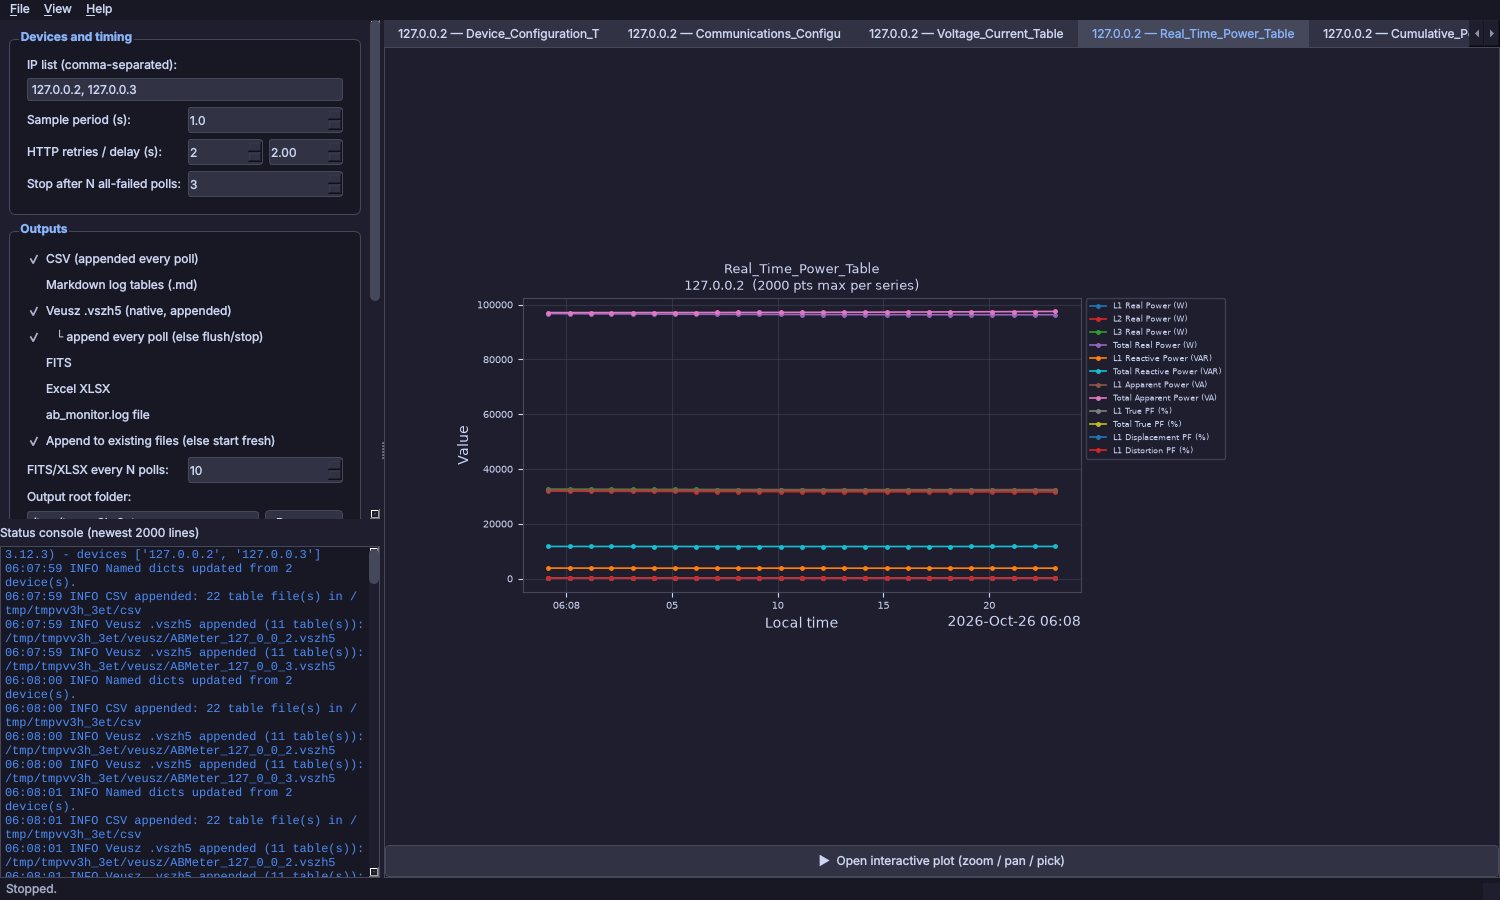
\includegraphics[width=\linewidth]{figures/gui_dark_1_6_0.png}
  \caption{Monitor 1.6.0 GUI, dark theme (off-screen capture, emulator data).}
  \label{fig:gui}
\end{figure}

% =============================================================================
\section{Deployment}
\subsection{Environment (mamba)}
\begin{lstlisting}[language=bash]
mamba env create -f environment.yml        # Python 3.12 + pip deps
mamba activate abmeter
# or pure conda-forge:
mamba env create -f environment-conda.yml
# Python 3.7.11 hosts:
mamba env create -f environment-py37.yml
\end{lstlisting}

\subsection{Services}
\begin{lstlisting}[language=bash]
sudo ./install.sh                     # headless monitor, system mode
sudo ./install.sh --exporter          # + Prometheus exporter
sudo ./install.sh --mamba             # mamba env, Python 3.12
python ab_stop.py                     # clean stop (STOP_COLLECTION)
\end{lstlisting}
{\sloppy The installer now also installs \code{vszh5_writer.py} and chooses
\code{requirements-py312.txt} on Python~$\ge$~3.12. The wrapper passes
\code{POLL_INTERVAL} and optional \code{RAM_PCT_LIMIT};
\code{ABMETER_OUTPUT_DIR} relocates the output.\par}

\subsection{Library use}
\begin{lstlisting}[language=Python]
import ab_power_meter_monitor as abm
cfg = abm.begin_run()                 # folders, log file, run bookkeeping
status = abm.poll_cycle(cfg)          # poll + store + persist + memory check
abm.perform_ram_flush(cfg, "manual")  # persist, then free rows
abm.end_run(cfg)                      # final writes (FITS/XLSX included)
\end{lstlisting}

% =============================================================================
\section{Configuration reference}
\begin{longtable}{@{}p{0.38\linewidth}p{0.12\linewidth}p{0.44\linewidth}@{}}
\toprule
Switch & Default & Meaning \\
\midrule
\endhead
\code{ENABLE_CSV}, \code{ENABLE_LOG_APPEND} & 0 & appended every poll \\
\code{ENABLE_VEUSZ} & 0 & native \code{.vszh5}, appended in place \\
\code{VEUSZ_APPEND_EVERY_CYCLE} & 1 & 0: append at flush/stop only \\
\code{ENABLE_FITS}, \code{ENABLE_XLSX} & 0 & rewritten atomically on a cadence \\
\code{FULL_WRITE_EVERY_N_CYCLES} & 10 & FITS/XLSX cadence (0: flush/stop) \\
\code{APPEND_OUTPUT_FILES} & 1 & 0: start files afresh once per run \\
\code{FSYNC_OUTPUTS} & 1 & fsync appended CSV/MD \\
\code{ENABLE_RAM_FLUSH} & 1 & automatic flush master switch \\
\code{MEM_FLUSH_THRESHOLD_MB} & 256 & $B_{\max}$ in Eq.~\ref{eq:trigger} \\
\code{MEM_PROC_RSS_LIMIT_MB} & 0 & $R_{\max}$ (0 = off) \\
\code{MEM_RAM_PCT_LIMIT} & 60 & $P_{\max}$ \\
\code{MEM_FREE_MIN_MB} & 512 & $M_{\min}$ \\
\code{MEM_MIN_STORE_MB_FOR_CLEAR} & 1.0 & $B_{\min}$ \\
\code{MEM_FLUSH_MIN_INTERVAL_SEC} & 120 & $T_{\min}$ \\
\code{RAM_FLUSH_KEEP_SAMPLES} & 0 & rows kept after a flush (GUI: 120) \\
\code{RAM_FLUSH_SPILL_PICKLE} & 0 & pickle the store when no output is on \\
\code{MEM_RETURN_TO_OS} & 1 & after a flush: \code{malloc_trim} / Windows heap decommit \\
\code{MEM_TRIM_WORKING_SET} & 1 & Windows: trim the working set after a flush \\
\code{VSZH5_MAX_FILE_MB} & 256 & \code{.vszh5} rollover \\
\code{VSZH5_TIME_AXIS} & local & \code{local} (DST-aware) or \code{utc} \\
\code{FITS_MAX_ROWS_PER_FILE} & 100000 & FITS rollover \\
\code{XLSX_MAX_ROWS_PER_FILE} & 50000 & XLSX rollover (Excel limit~\cite{excel_limits}) \\
\code{METER_URL_TEMPLATE} & see right & \code{http://{ip}/{page}}; proxy / emulator \\
\code{PREVIEW_MAX_POINTS} & 2000 & preview decimation \\
\code{GUI_LOG_MAX_LINES} & 2000 & console size \\
\bottomrule
\end{longtable}

% =============================================================================
\section{Verification}\label{sec:verification}
All tests run offline against \code{tests/ab_meter_emulator.py}, which serves
the 11 pages per host with drifting values, string cells, a duplicated
parameter name and optional faults. Python~3.12 runs used
\code{-W error::DeprecationWarning}. The Windows runs used the conda-forge
\code{win-64} build of Python~3.12.15 with numpy, h5py, astropy and openpyxl,
executed under Wine~9.0 with Microsoft's own \code{ucrtbase.dll}~\cite{wine}.

\begin{longtable}{@{}>{\raggedright\arraybackslash}p{0.30\linewidth}>{\raggedright\arraybackslash}p{0.46\linewidth}>{\raggedright\arraybackslash}p{0.17\linewidth}@{}}
\toprule
Test & What it proves & Result \\
\midrule
\endhead
\code{test_vszh5_appender} & create/append/reopen, NaN back-fill, layout conversion, real-Veusz render & pass (3.12, 3.8, Windows 3.12) \\
\code{test_monitor_offline} (8 tests) & one row per poll in every output across a flush; append across runs; fresh mode; FITS separation; duplicate names; trigger gating; locked \code{.vszh5}; no row sent twice to a busy writer; 23 pages render in Veusz 4.2.1 & pass (3.12, 3.8; Windows 3.12 three runs) \\
\code{test_memory_release} & bindings built once with 64-bit argument types; release never raises; flush of a \SI{98}{\mebi\byte} store returns it (Linux RSS 180 $\rightarrow$ 70 MiB); switch off; no overlap & pass (3.12, 3.8, Windows 3.12) \\
\code{test_exporter_offline} & no duplicate series; dead meter not exported; monotonic counters; \code{--timestamps}; SIGTERM shutdown (POSIX) & pass (3.12, 3.8; Windows 3.12 collector tests) \\
\code{gui_soak_test} (150\,s, 137--140 polls) & widget count constant (445; 447 with the 1.6.1 check boxes); previews rendered 137/137; no monitor errors; close waits for final writes & pass (3.12, 1.6.0 and 1.6.1) \\
\code{test_windows_file_locks} & files locked like Excel (\code{CreateFileW}, read-share): one warning per file, no error, rescue files on flush, merged back in order, no row lost or doubled & pass (3.12 Linux simulated; Windows 3.12 real locks) \\
\code{headless_soak_test} & real CLI, every output, automatic flushes, graceful stop; row counts equal in CSV, MD, \code{.vszh5}, XLSX, FITS; no leak & pass (3.12 Linux) \\
\code{run_all_tests} (Windows kit) & all suites + report + results zip & 8/8 pass (3.12 Linux, quick) \\
\code{test_windows_file_locks} & files locked like Excel (\code{CreateFileW}, read-share): one warning per file, no error, rescue files on flush, merged back in order, no row lost or doubled & pass (3.12 Linux simulated; Windows 3.12 real locks) \\
\code{headless_soak_test} & real CLI, every output, automatic flushes, graceful stop; equal row counts in CSV, MD, \code{.vszh5}, XLSX, FITS; no leak & pass (3.12 Linux) \\
\code{run_all_tests} (Windows kit) & all suites + report + results zip & 8/8 pass (3.12 Linux, quick) \\
Headless profile (600 polls, all outputs, flush every 50) & Python-traced memory constant; RSS plateau (Fig.~\ref{fig:headless}) & pass (3.12) \\
\bottomrule
\end{longtable}

\begin{figure}[ht]
  \centering
  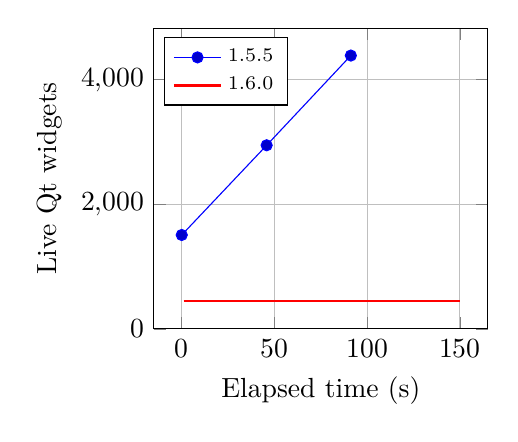
\begin{tikzpicture}
    \begin{axis}[width=0.48\linewidth,height=5.4cm,xlabel={Elapsed time (s)},
                 ylabel={Live Qt widgets},legend style={font=\scriptsize,at={(0.03,0.97)},anchor=north west},
                 grid=major,ymin=0]
      \addplot+[mark=*] coordinates {(0,1507)(45.8,2947)(91.2,4387)};
      \addlegendentry{1.5.5}
      \addplot+[mark=none,thick] coordinates {(1,445)(21,445)(47,445)(68,445)(90,445)(111,445)(133,445)(150,445)};
      \addlegendentry{1.6.0}
    \end{axis}
  \end{tikzpicture}\hfill
  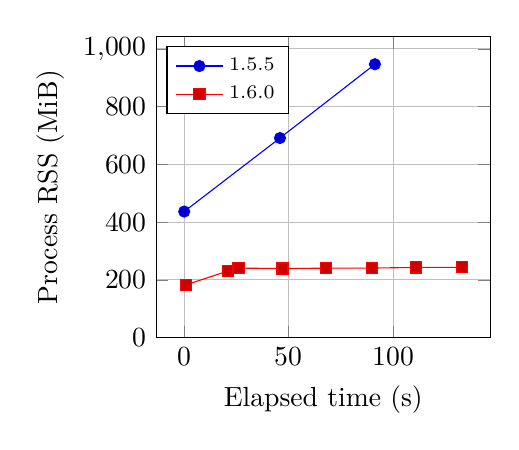
\begin{tikzpicture}
    \begin{axis}[width=0.48\linewidth,height=5.4cm,xlabel={Elapsed time (s)},
                 ylabel={Process RSS (MiB)},legend style={font=\scriptsize,at={(0.03,0.97)},anchor=north west},
                 grid=major,ymin=0]
      \addplot+[mark=*] coordinates {(0,436.4)(45.8,691.0)(91.2,946.5)};
      \addlegendentry{1.5.5}
      \addplot+[mark=square*] coordinates {(1,183.0)(21,230.7)(26,240.5)(47,239.1)(68,240.3)(90,240.8)(111,242.8)(133,243.1)};
      \addlegendentry{1.6.0}
    \end{axis}
  \end{tikzpicture}
  \caption{GUI soak, emulator, every output enabled. 1.5.5 at a 2\,s period;
  1.6.0 at a 1\,s period with tab switching, an interactive window and a
  Flush~RAM~Now during the run (elapsed time of 1.6.0 points approximated from
  poll count, 140 polls in 150\,s).}
  \label{fig:gui-leak}
\end{figure}

\begin{figure}[ht]
  \centering
  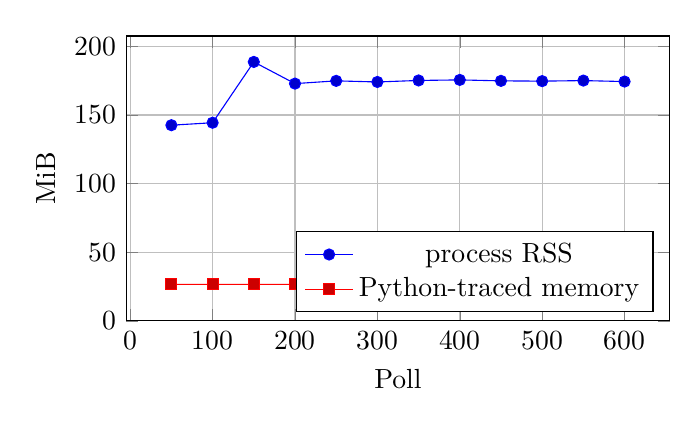
\begin{tikzpicture}
    \begin{axis}[width=0.7\linewidth,height=5.2cm,xlabel={Poll},ylabel={MiB},
                 legend pos=south east,grid=major,ymin=0]
      \addplot+[mark=*] coordinates {(50,142.6)(100,144.4)(150,188.7)(200,172.9)(250,174.9)(300,174.1)(350,175.2)(400,175.6)(450,174.9)(500,174.7)(550,175.1)(600,174.4)};
      \addlegendentry{process RSS}
      \addplot+[mark=square*] coordinates {(50,26.62)(100,26.63)(150,26.63)(200,26.63)(250,26.63)(300,26.63)(350,26.63)(400,26.63)(450,26.63)(500,26.63)(550,26.63)(600,26.63)};
      \addlegendentry{Python-traced memory}
    \end{axis}
  \end{tikzpicture}
  \caption{Headless monitor, 600 polls, CSV + Markdown + \code{.vszh5} every poll,
  FITS + XLSX every 25 polls, RAM flush every 50 polls (profiled with
  \code{tracemalloc}; the step at poll 150 is the profiler's own snapshot).}
  \label{fig:headless}
\end{figure}

% =============================================================================
\section{Module review}
\begin{longtable}{@{}p{0.2\linewidth}p{0.24\linewidth}p{0.48\linewidth}@{}}
\toprule
Module & Alternative & Decision \\
\midrule
\endhead
requests & httpx, urllib3 & kept; one keep-alive session per meter; HTTP/2 or async bring nothing to a single-threaded meter web server \\
beautifulsoup4 + lxml & \code{lxml.html} directly & kept: BeautifulSoup already parses with libxml2 through lxml; direct lxml text extraction can differ for nested markup and would rename columns in existing files. Trees are now \code{decompose()}'d \\
matplotlib (Agg) & pyqtgraph & kept for 1.6.0 (only the visible tab, decimated). pyqtgraph is the better long-term choice for live Qt plots (in-place \code{setData}, built-in downsampling, no PNG round trip) \\
openpyxl & XlsxWriter & kept, now read-only $\rightarrow$ write-only streaming~\cite{openpyxl_opt}; XlsxWriter is faster for pure writing but cannot read the existing workbook \\
astropy.io.fits & fitsio & kept (NRAO convention, no compiled extra) \\
veusz.embed & h5py + \code{vszh5_writer} & \textbf{replaced}: no Veusz process, in-place append, Python~3.12 wheels \\
psutil & /proc parsing & kept (cross-platform) \\
prometheus\_client & --- & kept; custom collector \\
qtpy + PySide6 & Qt.py & kept (the project's Qt abstraction layer) \\
\bottomrule
\end{longtable}

\noindent\textbf{GPU acceleration.} The workload is I/O bound (HTTP to embedded
meters, small appends); the only numeric kernels are min/max decimation and
array concatenation on at most tens of thousands of values per poll, which take
microseconds in NumPy. A GPU path would add a dependency without a measurable
benefit, so none was added.

\noindent\textbf{Python 3.12.} The interpreter's own improvements apply
without code changes, e.g. inlined comprehensions (PEP~709)~\cite{py312}; the
code avoids the APIs deprecated in 3.12.

% =============================================================================
\section{Known limitations and recommendations}
\begin{itemize}
  \item The Windows memory release was verified for binding, behaviour and
        error handling on Windows Python under Wine; the Task Manager drop
        itself follows from Microsoft's documented semantics and was not
        measured on a physical Windows machine for this release. Commit charge
        can stay above the working set when the heap is fragmented (it is
        re-used). On Windows~7 \code{HeapOptimizeResources} is not available
        (logged at DEBUG level); the working-set trim still works.
  \item The working-set trim makes pages still in use fault back in once
        (milliseconds). Setting \code{MEM_TRIM_WORKING_SET} to 0 leaves the
        working set to Windows.
  \item FITS and XLSX are rewrite formats; their cost grows with file size until
        rollover. Prefer CSV and \code{.vszh5} for long runs.
  \item FITS files written by 1.5.x with FITS enabled in the GUI may already
        contain mixed rows; start a new file.
  \item The local-time axis is ambiguous during the daylight-saving fall-back
        hour; \code{EPOCH_UTC} (FITS) and \code{VSZH5_TIME_AXIS = "utc"} avoid it.
  \item The interactive plot window's toolbar emits a matplotlib
        DeprecationWarning with PySide6 6.12 (third-party; harmless).
\end{itemize}

% =============================================================================
\begingroup\raggedright
\begin{thebibliography}{99}
\bibitem{qt_qtabwidget} The Qt Company, ``QTabWidget Class,'' \emph{Qt 6 Documentation}. [Online]. Available: \url{https://doc.qt.io/qt-6/qtabwidget.html} (accessed Oct. 26, 2026).
\bibitem{qt_qplaintextedit} The Qt Company, ``QPlainTextEdit Class,'' \emph{Qt 6 Documentation}. [Online]. Available: \url{https://doc.qt.io/qt-6/qplaintextedit.html} (accessed Oct. 26, 2026).
\bibitem{malloc_trim} M. Kerrisk \emph{et al.}, ``malloc\_trim(3),'' \emph{Linux man-pages}. [Online]. Available: \url{https://man7.org/linux/man-pages/man3/malloc_trim.3.html} (accessed Oct. 26, 2026).
\bibitem{h5py_datasets} h5py developers, ``Datasets,'' \emph{h5py documentation}. [Online]. Available: \url{https://docs.h5py.org/en/stable/high/dataset.html} (accessed Oct. 26, 2026).
\bibitem{veusz_src} J. Sanders \emph{et al.}, ``Veusz 4.2.1 source code,'' GitHub. [Online]. Available: \url{https://github.com/veusz/veusz} (accessed Oct. 26, 2026).
\bibitem{prom_exporters} Prometheus Authors, ``Writing exporters,'' \emph{Prometheus documentation}. [Online]. Available: \url{https://prometheus.io/docs/instrumenting/writing_exporters/} (accessed Oct. 26, 2026).
\bibitem{prom_query} Prometheus Authors, ``Querying basics: Staleness,'' \emph{Prometheus documentation}. [Online]. Available: \url{https://prometheus.io/docs/prometheus/latest/querying/basics/} (accessed Oct. 26, 2026).
\bibitem{prom_client} Prometheus Authors, ``Custom Collectors,'' \emph{prometheus\_client documentation}. [Online]. Available: \url{https://prometheus.github.io/client_python/collector/custom/} (accessed Oct. 26, 2026).
\bibitem{py_datetime} Python Software Foundation, ``datetime --- Basic date and time types,'' \emph{Python 3 documentation}. [Online]. Available: \url{https://docs.python.org/3/library/datetime.html} (accessed Oct. 26, 2026).
\bibitem{py312} Python Software Foundation, ``What's New In Python 3.12,'' \emph{Python 3 documentation}. [Online]. Available: \url{https://docs.python.org/3/whatsnew/3.12.html} (accessed Oct. 26, 2026).
\bibitem{openpyxl_opt} openpyxl developers, ``Optimised Modes,'' \emph{openpyxl documentation}. [Online]. Available: \url{https://openpyxl.readthedocs.io/en/stable/optimized.html} (accessed Oct. 26, 2026).
\bibitem{excel_limits} Microsoft, ``Excel specifications and limits,'' \emph{Microsoft Support}. [Online]. Available: \url{https://support.microsoft.com/en-us/excel/excel-specifications-and-limits} (accessed Oct. 26, 2026).
\bibitem{ms_heapsetinfo} Microsoft, ``HeapSetInformation function (heapapi.h),'' \emph{Microsoft Learn}. [Online]. Available: \url{https://learn.microsoft.com/en-us/windows/win32/api/heapapi/nf-heapapi-heapsetinformation} (accessed Oct. 26, 2026).
\bibitem{ms_emptyws} Microsoft, ``EmptyWorkingSet function (psapi.h),'' \emph{Microsoft Learn}. [Online]. Available: \url{https://learn.microsoft.com/en-us/windows/win32/api/psapi/nf-psapi-emptyworkingset} (accessed Oct. 26, 2026).
\bibitem{ms_heapcompact} Microsoft, ``HeapCompact function (heapapi.h),'' \emph{Microsoft Learn}. [Online]. Available: \url{https://learn.microsoft.com/en-us/windows/win32/api/heapapi/nf-heapapi-heapcompact} (accessed Oct. 26, 2026).
\bibitem{reactos_heapmin} ReactOS project, ``heapmin.cpp (Microsoft Universal CRT source),'' \emph{ReactOS Doxygen}. [Online]. Available: \url{https://doxygen.reactos.org/d1/ddd/heapmin_8cpp_source.html} (accessed Oct. 26, 2026).
\bibitem{moz_1553296} Mozilla, ``Bug 1553296: Decommit pages in the Windows system heap upon memory-pressure event,'' gecko-dev commit 0ef2cb2. [Online]. Available: \url{https://source-hub.etos-pro.ru/mozilla/gecko-dev/commit/0ef2cb2e18803ecbcc6419f337e151144c06cefa} (accessed Oct. 26, 2026).
\bibitem{cpython_futures} Python Software Foundation, ``Lib/concurrent/futures/\_base.py,'' CPython 3.12 source. [Online]. Available: \url{https://github.com/python/cpython/blob/3.12/Lib/concurrent/futures/_base.py} (accessed Oct. 26, 2026).
\bibitem{cpython_obmalloc} Python Software Foundation, ``Objects/obmalloc.c,'' CPython 3.12 source. [Online]. Available: \url{https://github.com/python/cpython/blob/3.12/Objects/obmalloc.c} (accessed Oct. 26, 2026).
\bibitem{wine} WineHQ, ``Wine 9.0,'' Ubuntu 24.04 package \code{wine64} 9.0\textasciitilde repack-4build3. [Online]. Available: \url{https://www.winehq.org/} (accessed Oct. 26, 2026).
\bibitem{ms_createfile} Microsoft, ``CreateFileW function (fileapi.h),'' \emph{Microsoft Learn}. [Online]. Available: \url{https://learn.microsoft.com/en-us/windows/win32/api/fileapi/nf-fileapi-createfilew} (accessed Oct. 26, 2026).
\bibitem{ms_ctrlevent} Microsoft, ``GenerateConsoleCtrlEvent function,'' \emph{Microsoft Learn}. [Online]. Available: \url{https://learn.microsoft.com/en-us/windows/console/generateconsolectrlevent} (accessed Oct. 26, 2026).
\bibitem{py_subprocess} Python Software Foundation, ``subprocess --- Subprocess management,'' \emph{Python 3 documentation}. [Online]. Available: \url{https://docs.python.org/3/library/subprocess.html} (accessed Oct. 26, 2026).
\bibitem{fits_std} IAU FITS Working Group, ``Definition of the Flexible Image Transport System (FITS), Version 4.0,'' 2018. [Online]. Available: \url{https://fits.gsfc.nasa.gov/fits_standard.html} (accessed Oct. 26, 2026).
\end{thebibliography}
\endgroup

\appendix
\section{Distribution contents}
\begin{tabularx}{\linewidth}{@{}lX@{}}
\toprule
Path & Content \\
\midrule
\code{*.py} (repository root) & monitor, writer, exporter, caller, examples, stop helper \\
\code{tests/} & meter emulator, offline, memory-release, file-lock and exporter tests, GUI and headless soaks, Windows memory check, test runner \\
\code{windows/} & Windows test kit (scripts, pinned specs, \code{START_HERE}) \\
\code{docs/} & this manual (LuaLaTeX source and PDF), figures \\
\code{requirements*.txt}, \code{environment*.yml} & dependencies (3.12 primary, 3.8+, 3.7) \\
\code{install*.sh}, \code{*.service}, wrapper & deployment kit \\
\code{patch/} & \code{git format-patch} series against \code{main} (7a9800b) \\
\bottomrule
\end{tabularx}
\end{document}
